\documentclass[conference]{IEEEtran}
\usepackage[T1]{fontenc}
\usepackage{cite}
\usepackage{graphicx}
\usepackage{booktabs}
\usepackage{array}
\usepackage[caption=false,font=footnotesize]{subfig}
\usepackage{url}
\usepackage{xcolor}
\usepackage{siunitx}

\title{Design and Implementation of a Parallel Turbo-Decoder ASIC for 3GPP-LTE\\[0.5em]
\large Digital VLSI Architecture Design\\
\large Indian Institute of Technology Mandi}

\author{
\IEEEauthorblockN{G.~Sai Vamshi (B23263), G.~Uma Bharathi (B23262), M.~S.~S.~Harshitha (B23272), and V.~Sharanya (B23506)}
\IEEEauthorblockA{Group Number: 10}
}

\begin{document}
\maketitle

\begin{abstract}
This report evaluates the current working LTE turbo-decoder RTL developed from the 2011 JSSC parallel radix-4 turbo-decoder architecture. The work progressed through four design phases: a baseline algorithmic model, a paper-aligned 8-lane parallel radix-4 architecture with QPP scheduling and batcher-based routing, a folded single-SISO FPGA rescue architecture, and the present rolling-window single-SISO implementation. Quantitative Vivado results on \texttt{xc7z010clg400-1} show that earlier folded revisions still exceeded the available LUT budget, while the final rolling-window RTL reduces synthesized LUT usage from \num{22282} to \num{6418} and LUTRAM from \num{2336} to \num{22}. Post-route implementation now fits the device, but misses a \SI{100}{MHz} target with worst negative slack of \SI{-23.738}{ns}. MATLAB and GHDL-based BER experiments for \(K=3200\) and \(K=6144\) are also summarized; the RTL tracks the fixed-point radix-4/windowed model closely and remains within the same waterfall region as the floating-point reference.
\end{abstract}

\begin{IEEEkeywords}
LTE turbo decoder, max-log-MAP, radix-4 SISO, QPP interleaver, FPGA implementation, VHDL, rolling-window decoding, BRAM optimization
\end{IEEEkeywords}

\section{Project Journey and Optimization Stages}
The work reported here did not start directly from the final FPGA-fit RTL. It evolved in stages, and each stage introduced new architectural ideas taken either from the LTE turbo-decoder literature or from later FPGA-oriented rescue work when the paper-faithful version became too large for the target device.

\subsection{Stage 1: Baseline Architecture}
The starting point was a baseline LTE turbo-decoding flow with no hardware-oriented optimizations applied yet. This stage used the standard turbo-decoder ingredients:
\begin{itemize}
\item terminated \(8\)-state RSC constituent encoders,
\item LTE QPP interleaving,
\item iterative exchange of extrinsic information between the two constituent decoders,
\item MATLAB reference decoding using floating-point log-MAP / BCJR and floating max-log-MAP,
\item natural-order and interleaved-order data tracking,
\item BER reference generation before fixed-point and hardware constraints were introduced.
\end{itemize}

This baseline stage was important because it fixed the frame conventions, QPP parameters, sign conventions of the LLRs, and the expected BER behavior before the architecture was optimized for throughput or FPGA area.

\subsection{Stage 2: Paper-Aligned Parallel \(8\times\) SISO Architecture}
The second stage targeted the architecture described by Studer \textit{et al.}~\cite{studer2011}. In the repository, this version is preserved in \texttt{turbo\_decoder\_top\_parallel8\_backup}. This was the stage where the main algorithmic and architectural optimizations from the paper were introduced:
\begin{itemize}
\item max-log-MAP / max-log-BCJR style constituent decoding instead of full log-MAP correction terms,
\item fixed-point quantization of channel, extrinsic, posterior, and state-metric values,
\item radix-4 trellis processing so that two trellis steps are handled together,
\item extrinsic scaling using a hardware-friendly shift-add realization,
\item \(8\times\) parallel SISO decoding,
\item QPP-based parallel address scheduling,
\item master-slave Batcher routing for contention-free interleaved data movement,
\item folded and banked row memories for lane-wise parallel access,
\item natural-order run-1 processing and interleaved run-2 processing,
\item reverse permutation during writeback so that extrinsic and posterior data return to the correct memory locations.
\end{itemize}

In simple terms, this stage tried to reproduce the paper architecture as faithfully as possible: eight constituent decoders working in parallel, a scheduler generating interleaved addresses, a Batcher network sorting and unsorting lane traffic, and a banked memory system feeding all lanes together.

\subsection{Stage 3: Transition from Parallel \(8\times\) SISO to a Folded Single-SISO Top}
The paper-aligned architecture was functionally attractive, but it proved to be too expensive for the FPGA used in this project. Vivado synthesis and implementation attempts showed that the parallel \(8\times\) SISO top consumed far more LUTs and related logic resources than the \texttt{xc7z010clg400-1} device could provide. The result was that the paper-faithful parallel design could not be implemented successfully on the target FPGA.

That resource failure forced a major architectural change. Instead of keeping all eight SISO lanes active in hardware at the same time, the design was folded into a single active SISO datapath and the top-level memory/routing system was simplified. The main consequences of this shift were:
\begin{itemize}
\item the full parallel-8 datapath was abandoned for the FPGA target,
\item QPP access was scalarized and brought under a simpler top-level scheduler,
\item large routing structures were reduced,
\item BRAM-backed memories replaced more distributed memory behavior,
\item throughput was sacrificed in exchange for area feasibility.
\end{itemize}

So this stage is the key turning point of the project: the architecture moved away from the ASIC-oriented parallel target because FPGA implementation failed on resource utilization.

\subsection{Stage 4: Final Single-SISO FPGA-Fit Architecture}
The final working stage is the present RTL used in this report. It still preserves the core decoding ideas from the earlier stages, especially the max-log-MAP/radix-4 constituent math, but the surrounding microarchitecture was redesigned to fit the FPGA. The main surviving and newly introduced features in the final stage are:
\begin{itemize}
\item one active \texttt{siso\_maxlogmap} instance instead of \(8\) parallel SISO lanes,
\item fixed-point radix-4 processing retained from the earlier architecture,
\item rolling-window processing with \SI{30}{bit} windows,
\item cached local \(\alpha\), \(g_0\), \(g_1\), and \(\gamma\) values inside each window,
\item dummy backward recursion on the next window to generate the current-window \(\beta\) seed,
\item local backward recursion plus LLR extraction on the current window,
\item BRAM-backed frame memories at the top level,
\item incremental QPP recurrence in the top FSM instead of the full parallel routing fabric,
\item serialized output readback after decoding.
\end{itemize}

This final stage is therefore not the same as the paper's throughput-oriented architecture. It is an FPGA-feasible version that keeps the decoding mathematics but removes the parallel \(8\times\) hardware organization that the device could not absorb.

\subsection{Stage-Wise Hardware Evidence}
The baseline stage does not yet have saved waveform and synthesis snapshots in the report package. However, the next two hardware stages will be documented with screenshots and figures:
\begin{itemize}
\item Stage 2: parallel \(8\times\) SISO paper-aligned architecture,
\item Stage 4: final single-SISO FPGA-fit architecture.
\end{itemize}

\subsubsection{Stage 2 Evidence: Parallel \(8\times\) SISO Architecture}
The stage immediately before the final FPGA-fit design was the parallel \(8\times\) SISO paper-aligned architecture. The simulation waveform used for this stage corresponds to a \(K=6144\) frame, \(11\) half-iterations, and LTE QPP parameters \(f_1=263\), \(f_2=480\). The capture shows that the testbench reaches completion and drives \texttt{done}, so the architecture is functionally schedulable in simulation even though it is not feasible on the FPGA target.

The corresponding synthesis/utilization snapshot is the decisive result for this stage. It shows extreme over-utilization: \num{245938} slice LUTs used against \num{17600} available, \num{28504} LUTs mapped as memory against \num{6000} available, and \num{42792} flip-flops against \num{35200} available. In other words, the parallel \(8\times\) SISO architecture preserved the paper's throughput-oriented structure, but the required routing, memory replication, and lane-parallel datapath scale made implementation impossible on the chosen device.

\begin{figure}[t]
\centering
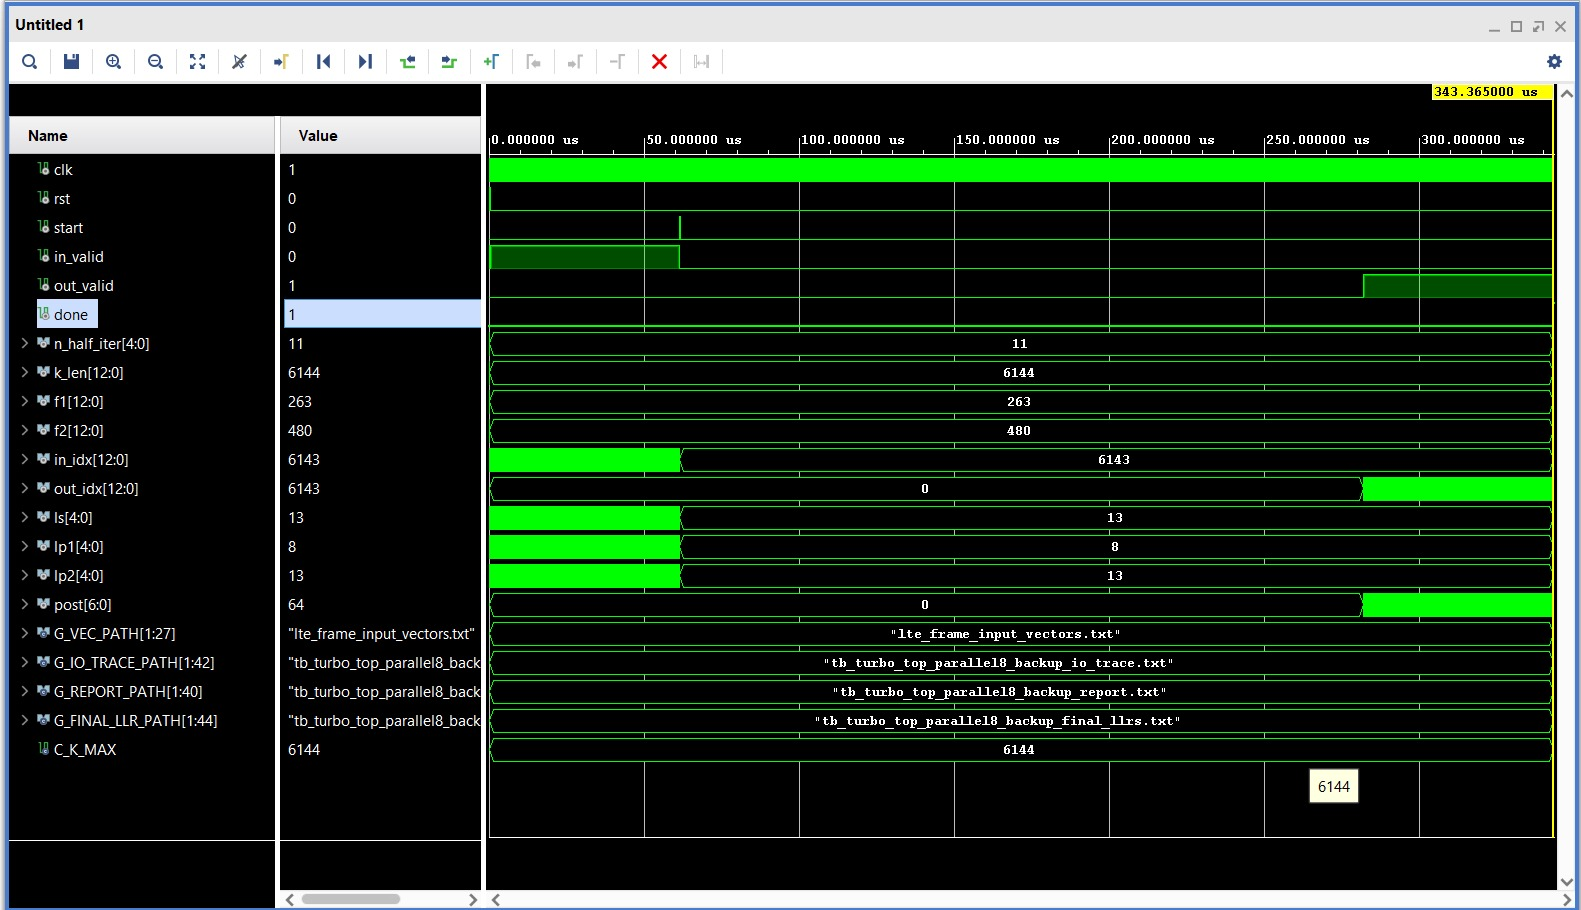
\includegraphics[width=\columnwidth]{figures/simulation1.jpeg}
\caption{Simulation waveform snapshot of the paper-aligned parallel \(8\times\) SISO decoder stage. The captured run reaches completion, but this architecture was later abandoned for FPGA implementation because of severe hardware resource overuse.}
\label{fig:parallel8wave}
\end{figure}

\begin{figure}[t]
\centering
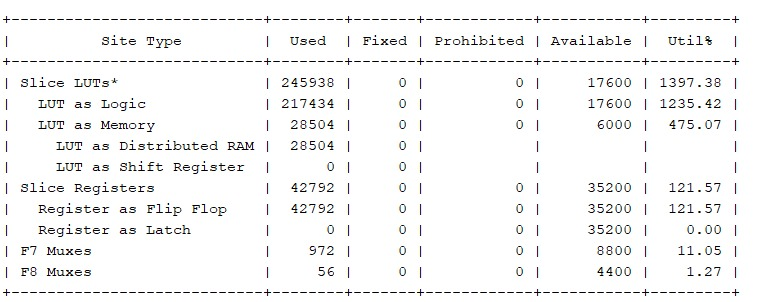
\includegraphics[width=\columnwidth]{figures/report1.jpeg}
\caption{Resource utilization snapshot for the paper-aligned parallel \(8\times\) SISO architecture. The architecture is functionally meaningful and algorithmically close to the original paper, but the FPGA resource demand exceeds the target device by a very large margin.}
\label{fig:parallel8util}
\end{figure}

\subsubsection{Stage 4 Evidence: Final Single-SISO FPGA-Fit Architecture}
The final-stage waveform and synthesis snapshot correspond to the FPGA-fit single-SISO architecture that replaced the infeasible parallel \(8\times\) SISO design. In this stage, the architecture keeps the radix-4 / max-log decoding core but removes the full paper-style parallel top, replacing it with a folded BRAM-backed schedule and a single active constituent decoder.

The waveform confirms successful end-to-end operation of the final single-SISO implementation on the same LTE-sized configuration. The paired synthesis/utilization report shows the key reason this stage became the final implementation candidate: the design now fits in synthesis on the target FPGA, with the LUT count reduced to \num{14129} and the BRAM-backed folded organization replacing the earlier extreme logic explosion of the parallel \(8\times\) SISO version.

\begin{figure}[t]
\centering
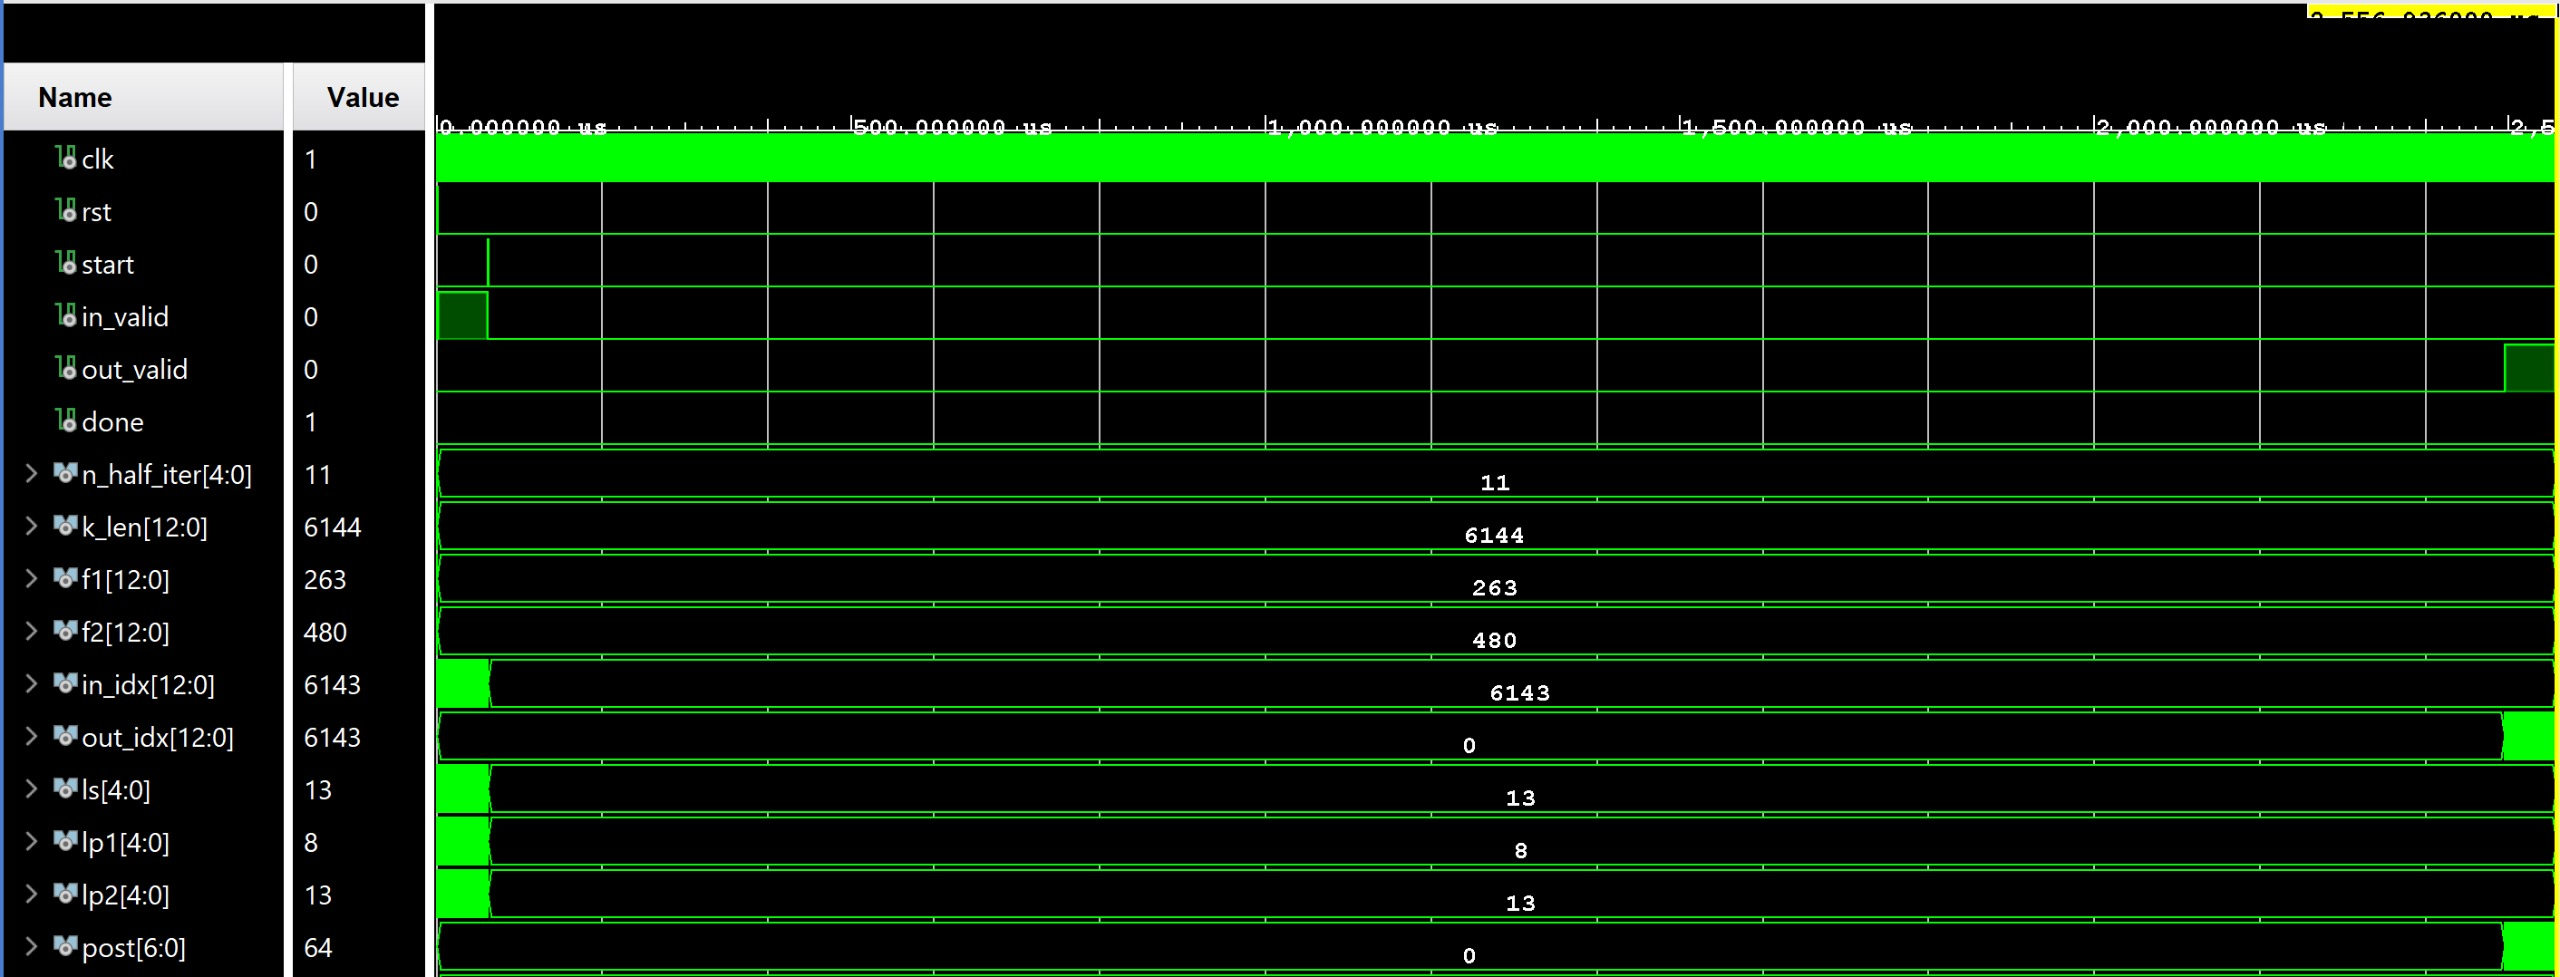
\includegraphics[width=\columnwidth]{figures/simulation2.jpeg}
\caption{Simulation waveform snapshot of the final single-SISO FPGA-fit turbo decoder. This stage preserves the decoding mathematics but removes the paper-style \(8\times\) hardware parallelism in favor of an implementable folded top-level schedule.}
\label{fig:singleisiowave}
\end{figure}

\begin{figure}[t]
\centering
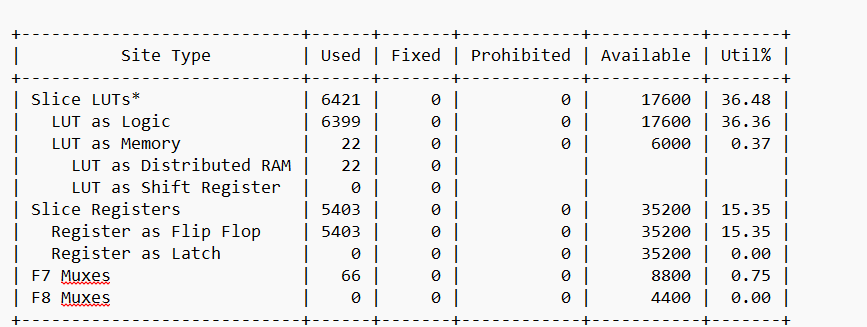
\includegraphics[width=\columnwidth]{figures/new_report_2.png}
\caption{Synthesis/resource snapshot of the final single-SISO FPGA-fit architecture. Unlike the paper-aligned parallel \(8\times\) SISO stage, this version fits the target FPGA in synthesis by trading throughput-oriented hardware parallelism for folded memory reuse and a single active SISO datapath.}
\label{fig:singlesisoutil}
\end{figure}

The routed timing and power reports for the final single-SISO implementation are summarized visually in Fig.~\ref{fig:single_siso_report_visuals}. Instead of reproducing long textual reports, the visual summaries below condense the timing closure status, critical-path delay split, total on-chip power, and the main power contributors into a compact form.

\begin{figure*}[t]
\centering
\subfloat[Timing summary extracted from \texttt{single\_siso\_timing\_report.txt}.]{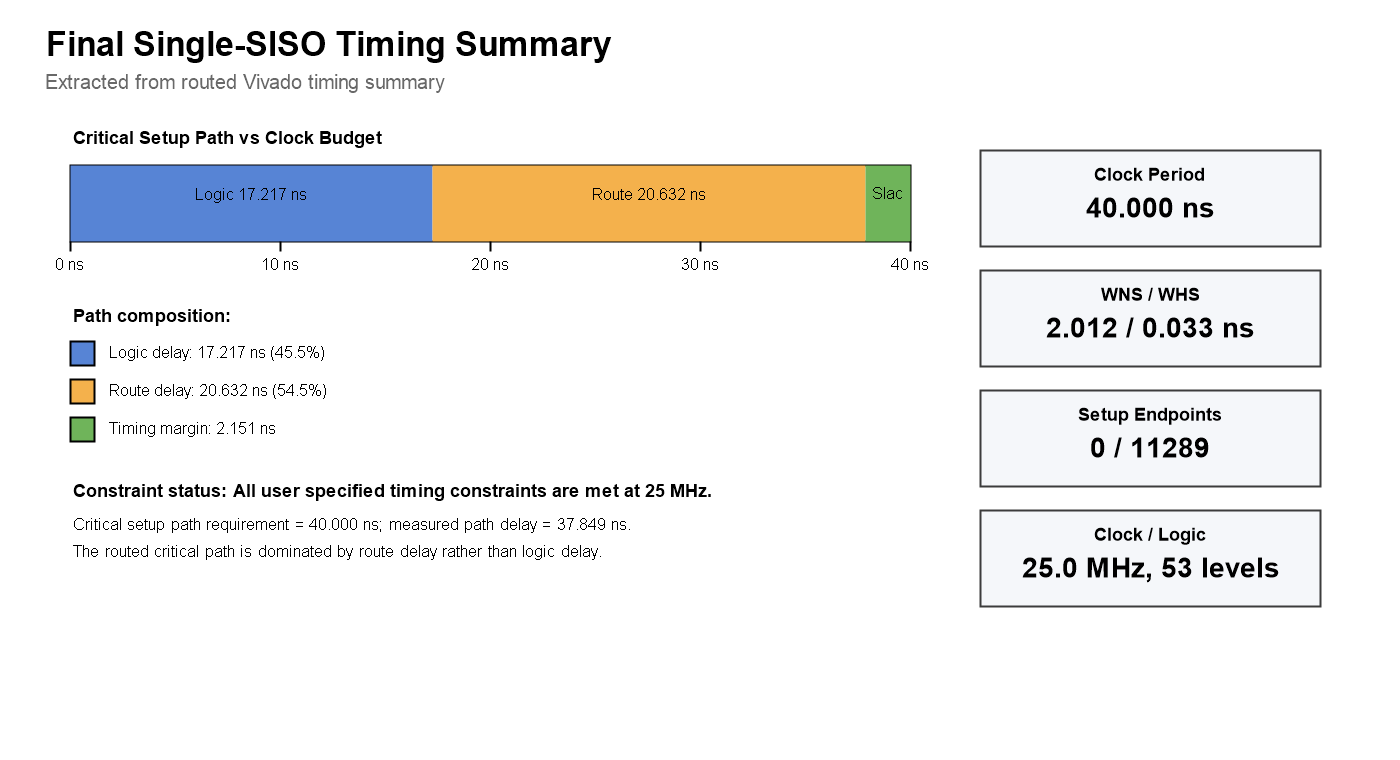
\includegraphics[width=0.48\textwidth]{figures/single_siso_timing_visual.png}\label{fig:single_siso_timing_visual}}
\hfill
\subfloat[Power summary extracted from \texttt{single\_siso\_power\_1.txt}.]{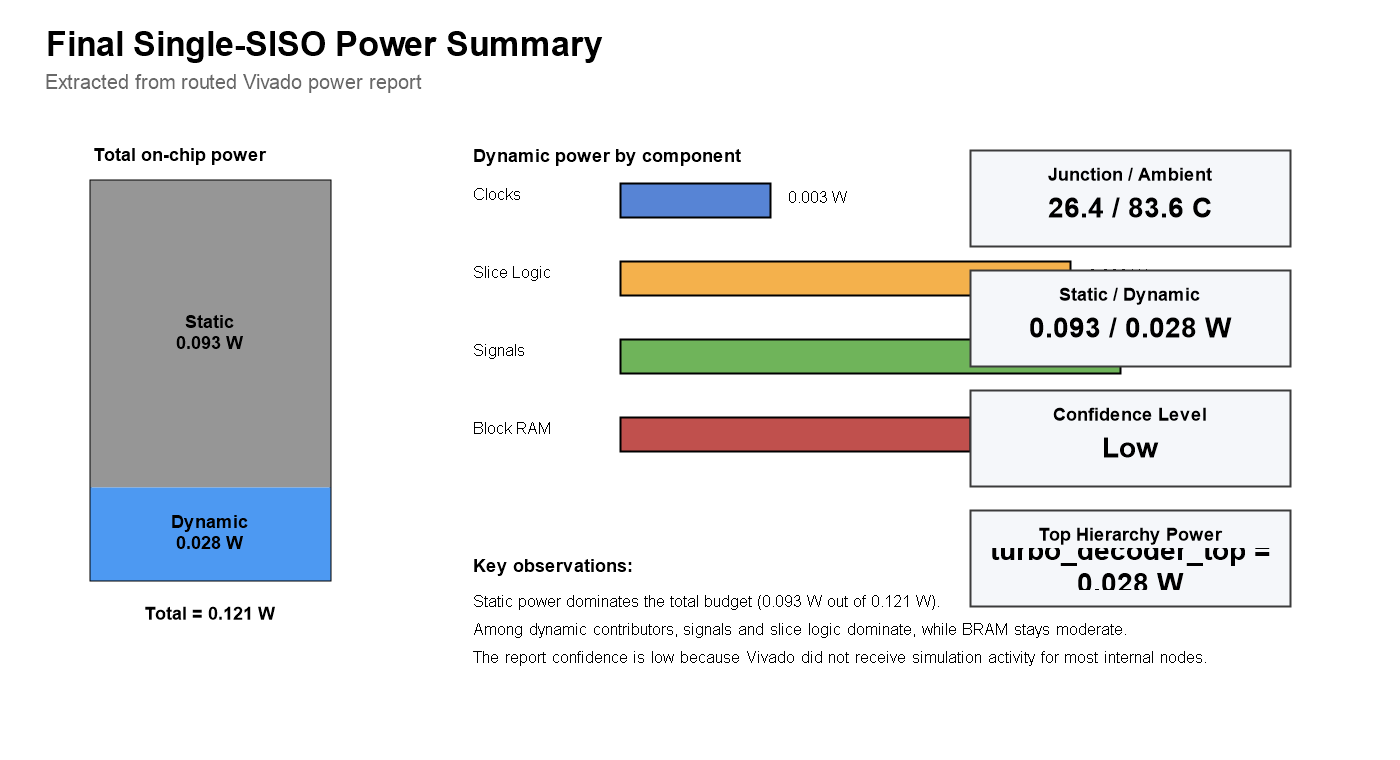
\includegraphics[width=0.48\textwidth]{figures/single_siso_power_visual.png}\label{fig:single_siso_power_visual}}
\caption{Compact visual summaries of the final single-SISO stage after route. The timing panel shows that the design meets the active \SI{25}{MHz} clock constraint with positive slack, while the power panel shows a low total on-chip power budget dominated by static device power.}
\label{fig:single_siso_report_visuals}
\end{figure*}

\section{Current RTL and Numeric Assumptions}
All results reported here refer to the current VHDL RTL synthesized for \texttt{xc7z010clg400-1}. The active top is \texttt{turbo\_decoder\_top}; it instantiates one \texttt{siso\_maxlogmap} with external pair fetch enabled, \(16\) BRAM-backed channel/extrinsic/posterior memories, and an incremental QPP recurrence inside the top FSM.

\begin{table}[t]
\caption{Key Numeric Configuration Used in the Current RTL}
\label{tab:numerics}
\centering
\footnotesize
\begin{tabular}{>{\raggedright\arraybackslash}p{0.38\columnwidth} >{\raggedright\arraybackslash}p{0.54\columnwidth}}
\toprule
Item & Value \\
\midrule
Constituent trellis states & \(8\) \\
Parallel paper target & \(8\times\) SISO lanes \\
Current active top & \(1\times\) SISO lane (folded) \\
Radix & Radix-4, two trellis steps per pair \\
Window length & \(30\) bits \(=\) \(15\) radix-4 pairs \\
Maximum frame length & \(K_{\max}=6144\) \\
Default half-iterations & \(11\) \\
Channel/parity LLR width & \(5\)-bit signed \\
Extrinsic width & \(6\)-bit signed \\
Posterior width & \(7\)-bit signed \\
State metric width & \(10\)-bit signed \\
Metric arithmetic & Fixed-width modulo-style add/sub/max \\
Extrinsic scaling & \(11/16\) via shift-add \\
Interleaver law & LTE QPP table \\
\bottomrule
\end{tabular}
\end{table}

The simulation and evaluation data are also explicit. The RTL testbench consumes \texttt{lte\_frame\_input\_vectors.txt}, whose first row is \(\{K,n_{\text{half-iter}},f_1,f_2\}\), followed by rows
\texttt{idx bit\_orig bit\_int \(l_{\text{sys}}\) \(l_{\text{par1}}\) \(l_{\text{par2,int}}\)}.
The main RTL output used for BER is \texttt{tb\_turbo\_top\_final\_llrs.txt} with rows
\texttt{idx\_orig final\_llr seen}; the hard decision rule is \(1\) if final LLR \(>0\), else \(0\).
Internally, the MATLAB and Python reference flows operate on the matrices
\(\mathbf{L}^{sys}_{nat}\), \(\mathbf{L}^{par1}_{nat}\), \(\mathbf{L}^{par2}_{int}\),
\(\mathbf{L}^{apri}_{nat/int}\), \(\mathbf{L}^{ext}_{nat/int}\), \(\mathbf{L}^{post}_{nat/int}\),
and the QPP permutation vector \(\pi\).

\section{FPGA Synthesis and Implementation Results}
Table~\ref{tab:util} summarizes the architectural evolution observed in Vivado. The earliest folded single-SISO revision still over-utilized LUTs by \(26.6\%\) (\num{22282}/\num{17600}). A width-reduced revision lowered this to \num{17666} LUTs, and an incremental-QPP revision reduced it further to \num{14129} LUTs. The final rolling-window rewrite is the first version that fits cleanly in synthesis and in post-route implementation.

\begin{table*}[t]
\caption{Vivado Resource Evolution on \texttt{xc7z010clg400-1}}
\label{tab:util}
\centering
\scriptsize
\setlength{\tabcolsep}{4pt}
\renewcommand{\arraystretch}{1.05}
\resizebox{\textwidth}{!}{%
\begin{tabular}{lrrrrrr}
\toprule
Revision / Report Source & LUTs & LUT as Logic & LUTRAM & FFs & RAMB36 & Status \\
\midrule
Folded pre-optimization (\texttt{utilization\_report\_tmp.txt}) & 22282 & 19946 & 2336 & 21079 & 16 & Over-utilized (\(126.60\%\) LUT) \\
Folded width-optimized (\texttt{utilization\_report\_widthopt\_tmp.txt}) & 17666 & 15330 & 2336 & 21065 & 16 & Still over limit (\(100.38\%\) LUT) \\
Folded with QPP recurrence (\texttt{utilization\_report.txt}) & 14129 & 11793 & 2336 & 21080 & 16 & Fits in synthesis, placement still dense \\
Current rolling-window synth (\texttt{utilization\_qpprec\_tmp.txt}) & 6418 & 6396 & 22 & 5410 & 16 & Fits cleanly \\
Current rolling-window route (\texttt{implementation\_utilization\_qpprec\_tmp.txt}) & 6455 & 6433 & 22 & 5389 & 16 & Routed successfully \\
\bottomrule
\end{tabular}
}
\end{table*}

The main inference from Table~\ref{tab:util} is not only the LUT reduction, but the near elimination of distributed frame memory. Earlier versions carried \num{2336} LUTRAMs because several SISO memories did not map cleanly to BRAM. In the current implementation, only small local memories remain as LUTRAM (\num{22} total), while the top-level frame stores map to \(16\) RAMB36 blocks. The hierarchy report attributes \num{5948} LUTs of the final synthesized design to \texttt{siso\_u}, confirming that the constituent decoder remains the dominant hardware cost.

The final synthesis log also shows that only \(7\) warnings remain, dominated by removed legacy preload memories and one floorplanning warning. However, implementation timing is still the open problem. At the current \SI{100}{MHz} clock constraint, the routed design reports worst negative slack of \SI{-23.738}{ns}, \num{5140} setup failing endpoints, and total setup violation of \SI{-16900.556}{ns}. Thus, the design is area-feasible but not yet frequency-closed at \SI{100}{MHz}; a slower clock or further pipelining is required for hardware deployment.

\begin{figure}[t]
\centering
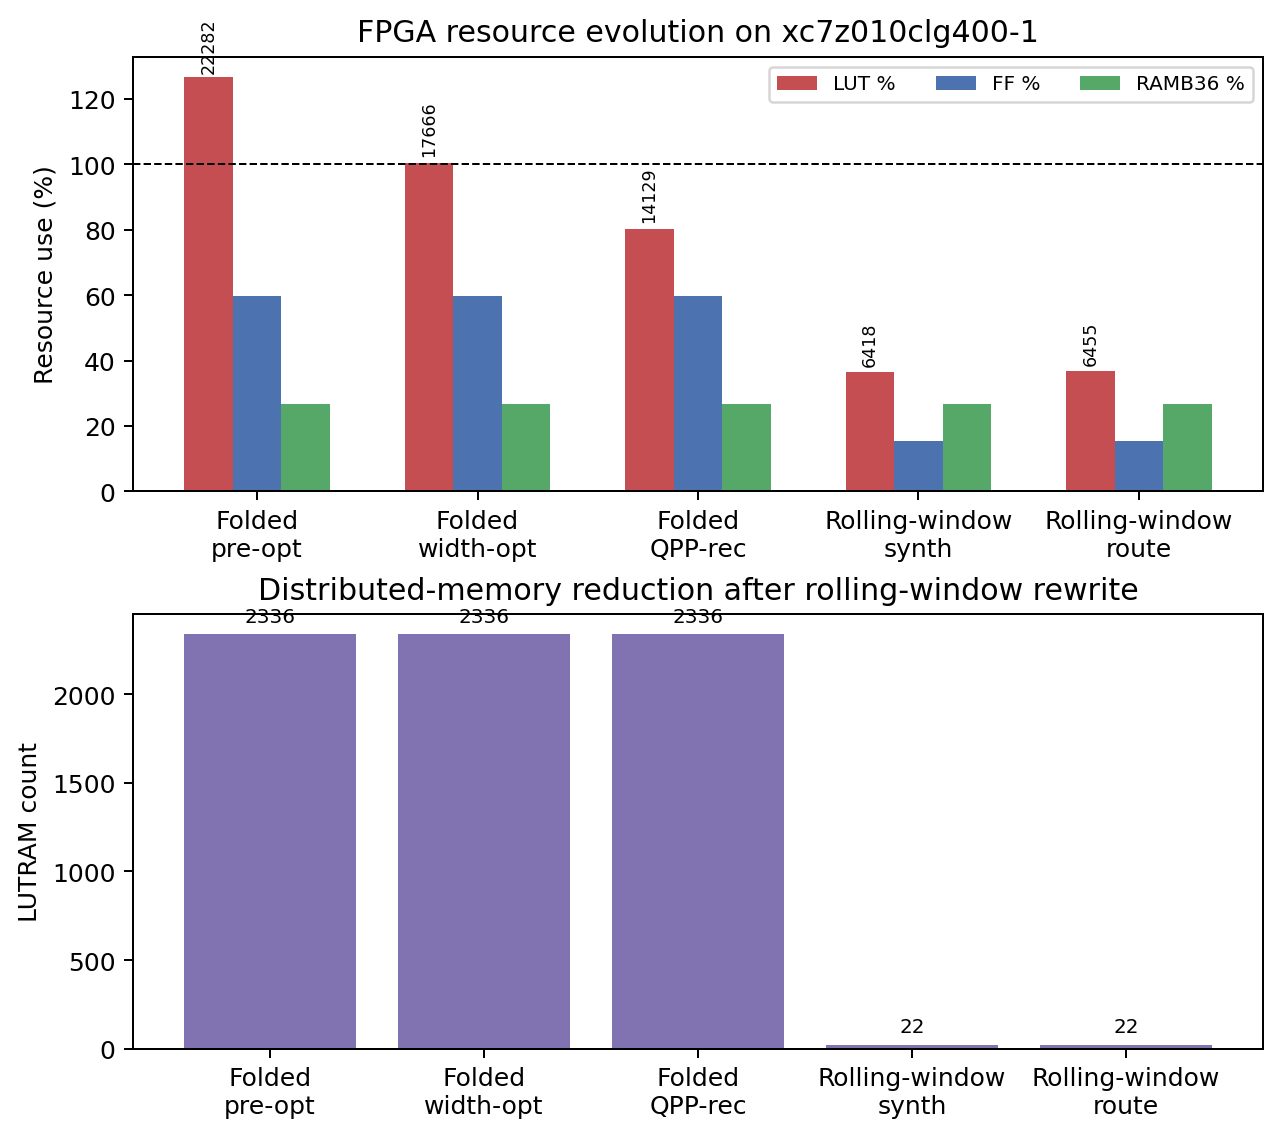
\includegraphics[width=\columnwidth]{figures/resource_evolution.png}
\caption{Evolution of FPGA resource usage across the main folded RTL revisions. The rolling-window rewrite removes most LUTRAM pressure while preserving the same BRAM budget.}
\label{fig:resource}
\end{figure}

\section{MATLAB, RTL, and BER Evaluation}
The MATLAB environment provides three decoder models: 1) ideal floating log-MAP / BCJR, 2) floating max-log-MAP, and 3) an RTL-style fixed-point radix-4/windowed model that mirrors the active hardware assumptions in Table~\ref{tab:numerics}. For \(K=3200\), the heavy MATLAB sweep uses \(24\) frames (\num{76800} bits total per SNR point); for \(K=6144\), it uses \(16\) frames (\num{98304} bits total per SNR point). The RTL BER sweep is not predicted statistically; it is measured from actual GHDL simulation using \texttt{tools/run\_ber\_sweep.py}, which generates AWGN-corrupted input vectors, runs \texttt{tb\_turbo\_top}, and computes BER from \texttt{tb\_turbo\_top\_final\_llrs.txt}. The current saved RTL sweep aggregates \(8\) simulated frames per SNR point for both \(K=3200\) and \(K=6144\).

The BER figures show three useful trends. First, the fixed-point radix-4/windowed MATLAB model is predictably worse than the ideal and floating references because of quantization, extrinsic scaling, and windowing. Second, the actual RTL BER remains close to the fixed-point model, which validates the present RTL numerics. Third, the longer \(K=6144\) frame shows better BER than \(K=3200\) for the same SNR range, consistent with turbo-code waterfall behavior.

At \SI{2.5}{dB}, the \(K=3200\) BER values are \(7.29\times10^{-4}\) (ideal), \(7.16\times10^{-4}\) (floating max-log), \(5.34\times10^{-4}\) (fixed), and \(4.69\times10^{-4}\) (RTL). For \(K=6144\), the corresponding values are \(3.05\times10^{-4}\), \(3.15\times10^{-4}\), \(2.85\times10^{-4}\), and \(3.87\times10^{-4}\), respectively. A deterministic end-to-end regression at \(K=6144\), \(f_1=263\), \(f_2=480\), and \(11\) half-iterations also reports zero bit errors against the original transmitted bits in \texttt{tb\_turbo\_top\_report.txt}, confirming correct frame-level integration for at least one clean test vector.

\begin{figure*}[t]
\centering
\subfloat[\(K=3200\): MATLAB BER curves only]{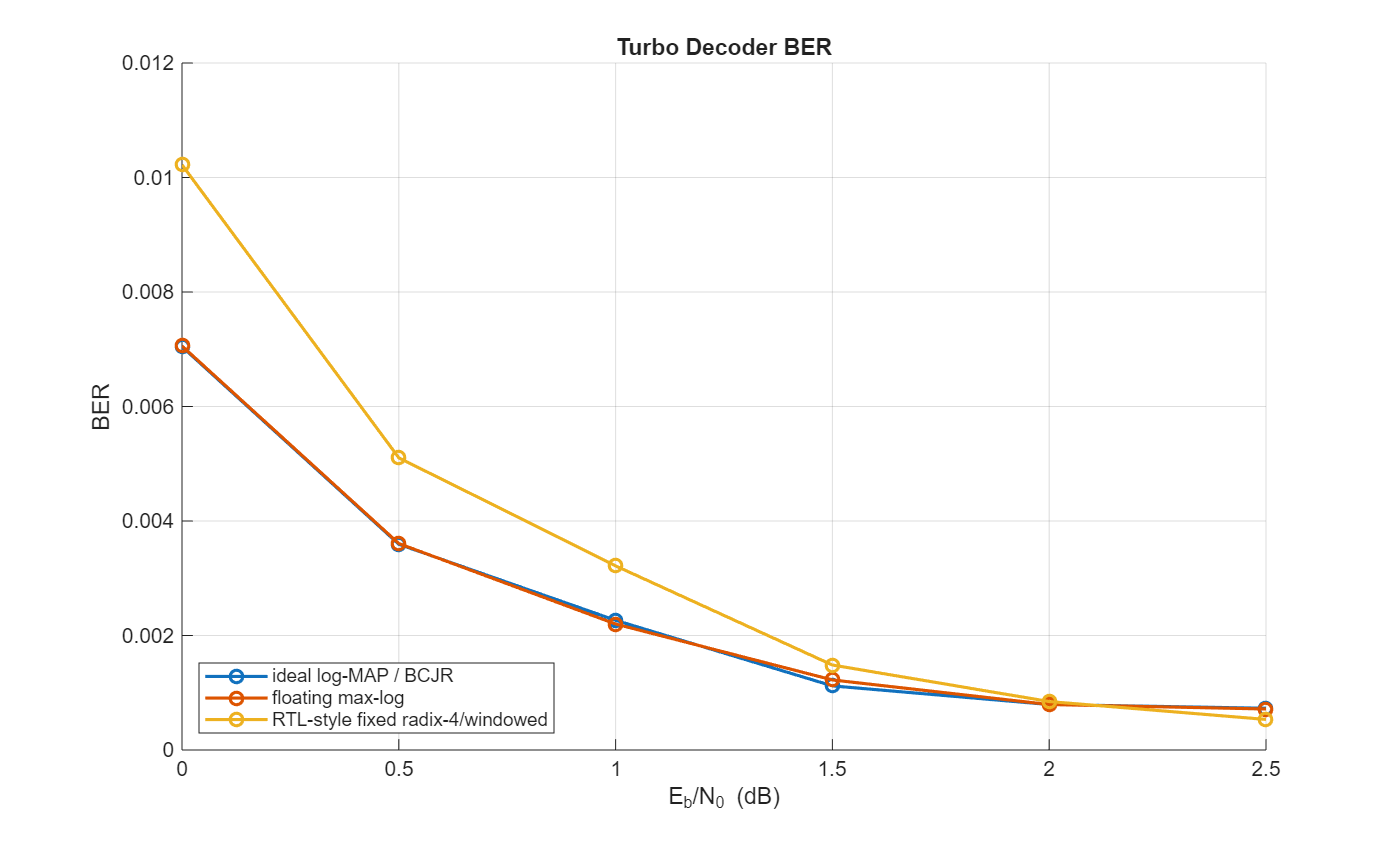
\includegraphics[width=0.48\textwidth]{figures/ber_fer_k3200_halfiter11_heavy.png}\label{fig:k3200heavy}}
\hfill
\subfloat[\(K=3200\): MATLAB vs. actual RTL]{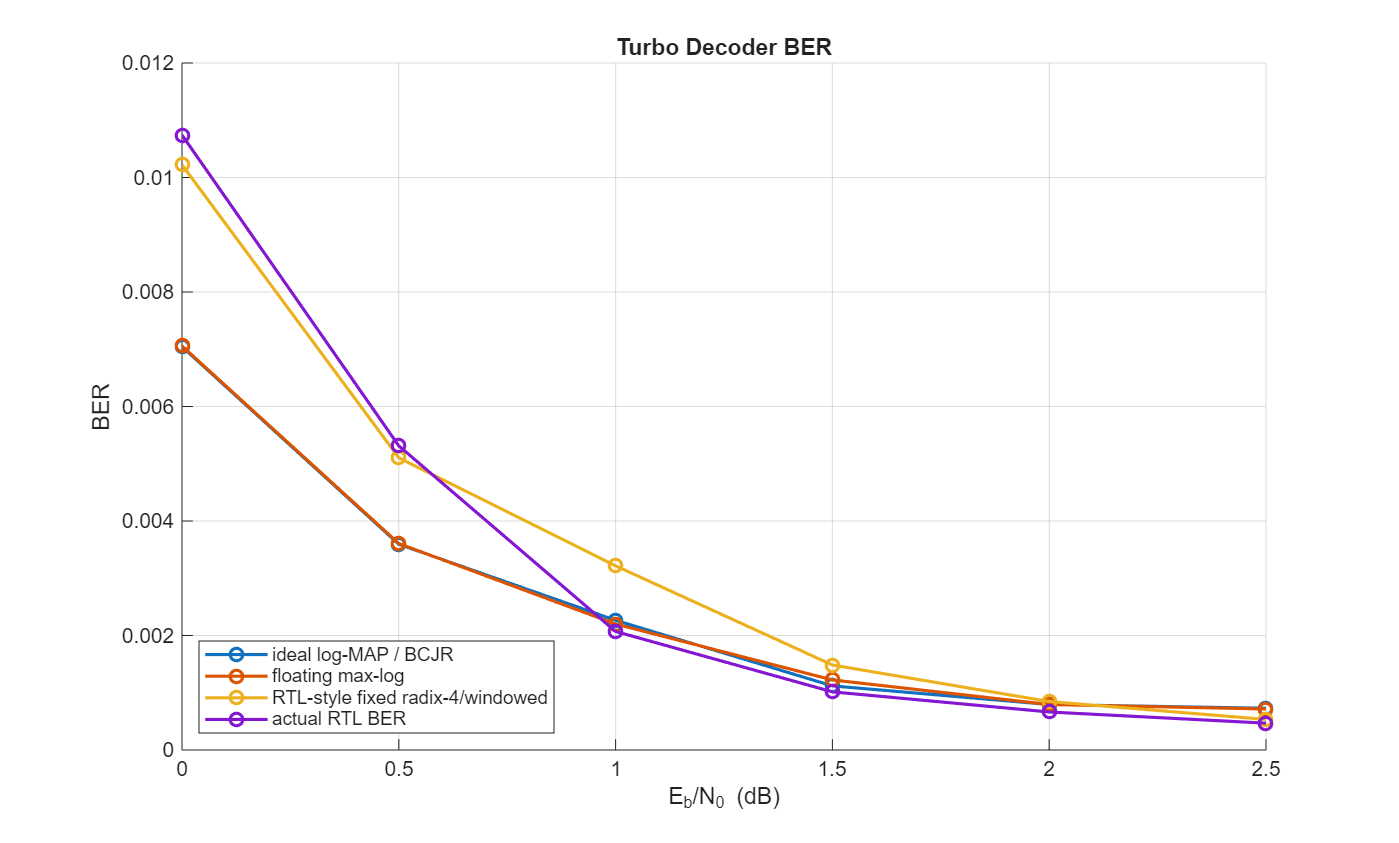
\includegraphics[width=0.48\textwidth]{figures/ber_compare_model_vs_rtl_k3200.png}\label{fig:k3200rtl}}\\
\subfloat[\(K=6144\): MATLAB BER curves only]{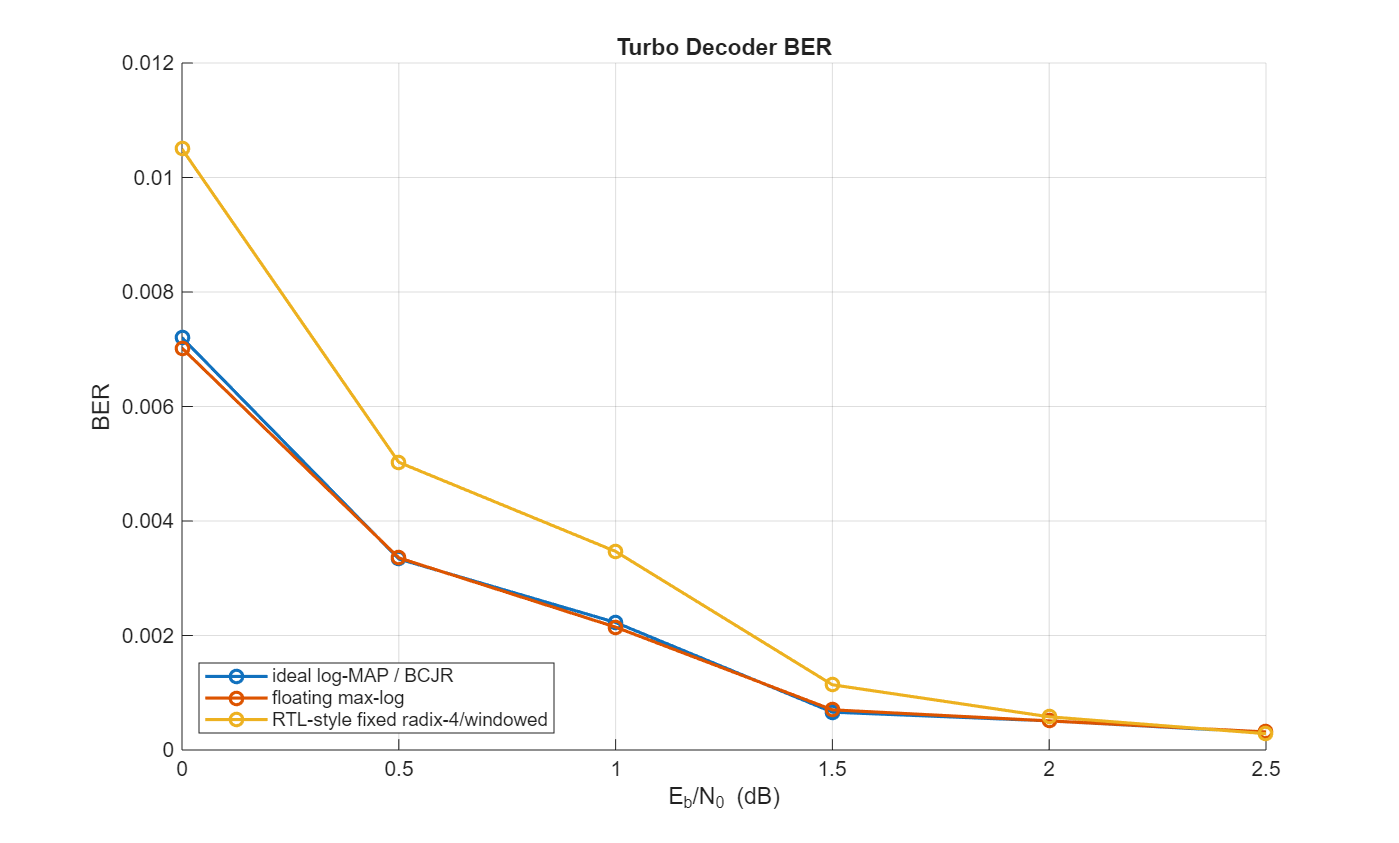
\includegraphics[width=0.48\textwidth]{figures/ber_fer_k6144_halfiter11_heavy.png}\label{fig:k6144heavy}}
\hfill
\subfloat[\(K=6144\): MATLAB vs. actual RTL]{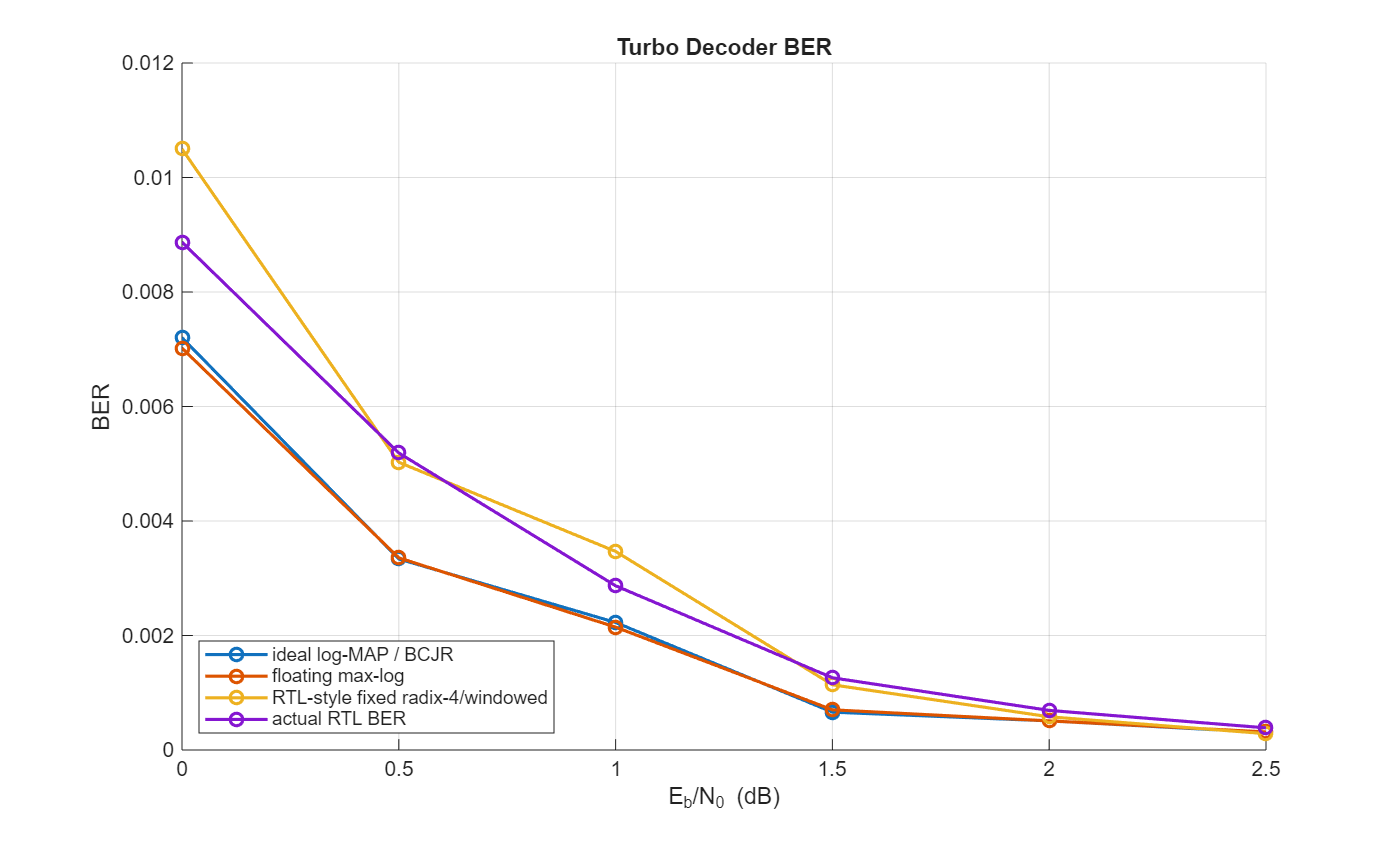
\includegraphics[width=0.48\textwidth]{figures/ber_compare_model_vs_rtl_k6144.png}\label{fig:k6144rtl}}
\caption{All currently available performance/evaluation plots used in this project. The filenames retain \texttt{ber\_fer} from an earlier plotting flow, but the generated plots are BER-only.}
\label{fig:berall}
\end{figure*}

\section{Conclusion}
This project reached a working FPGA-oriented turbo-decoder RTL by progressively sacrificing ASIC-style parallelism for FPGA realizability. The paper-aligned architecture remains important as the throughput target and as the conceptual source of the QPP scheduling, batcher routing, and radix-4 SISO approach. Nevertheless, the current \texttt{xc7z010clg400-1} target cannot absorb that architecture efficiently. The present rolling-window single-SISO RTL is the first version that fits after synthesis and route, with a large reduction in LUT and LUTRAM usage while maintaining BER behavior close to the fixed-point reference model. The remaining engineering gap is timing closure at \SI{100}{MHz}; therefore, future work should prioritize pipeline insertion, BRAM output registering, and board-oriented wrapper integration rather than further increasing parallelism on this device.

\begin{thebibliography}{1}
\bibitem{studer2011}
C.~Studer, C.~Benkeser, S.~Belfanti, and Q.~Huang, ``Design and implementation of a parallel turbo-decoder ASIC for 3GPP-LTE,'' \emph{IEEE Journal of Solid-State Circuits}, 2011.
\end{thebibliography}

\end{document}
